%Put this in order they appear in beamline?
\section{Tritium Target System}

When the beam reaches the center of Hall A, it will meet the target. Here the beam will either interact with the target and scatter, allowing for detection of events that are within the acceptance of the spectrometer, or pass through the target and be deposited in the beam dump. Figure \ref{fig:ha_side} shows a side view of the hall, with the beam going from left to right. This view of the hall clearly shows these two possible paths for the beam (along the dashed line). For clarity, the spectrometer is drawn at a $0\degree$ scattering angle, which is not a position the spectrometer can physically occupy.

\begin{figure}
\begin{center}
	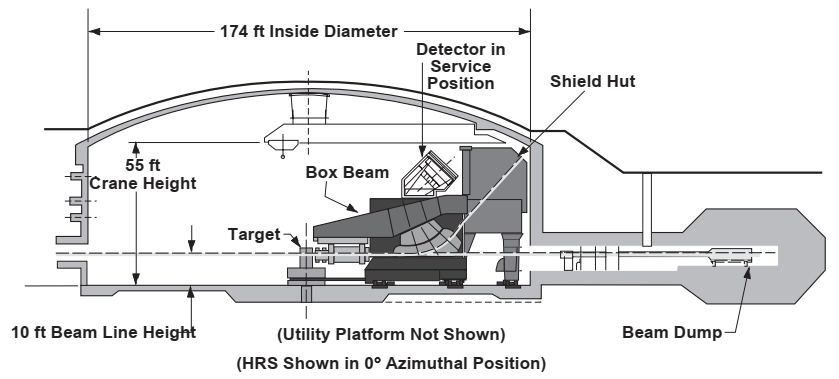
\includegraphics[width=.8\textwidth]{./setup/fig/HallA_side.png}
	\caption{A side-view schematic of Hall A showing the beamline, target, High Resolution Spectrometers, and Beam Dump. The beam will either interact with the target or pass through to the beam dump.\cite{HANIM}}
	\label{fig:ha_side}
\end{center}
\end{figure}

\subsection{Gas Cell Design}
\label{sec:gas_cell}
The gas targets used in this experiment were housed in a specially designed cell. This cell deviates from typical cells used in Hall A in that the gas is not circulated. The need for such a design is to meet safety protocols when using a tritium target, specifically to minimize tritium material and to mitigate the risk of tritium leakage.

The target cells are 25 centimeters long and made of Aluminum 7075. The cells are sealed and utilize conductive cooling. The beam heating of the aluminum is approximately 11W. This heat is recovered by a copper heat sink that is actively cooled by 15K helium gas.\cite{cell_design} Figure \ref{fig:3d_cell} shows a 3-dimensional rendering of the target cell. The beam comes in from the bottom-left and passes through the center of the target along the length.

\begin{figure}[h]
\begin{center}
	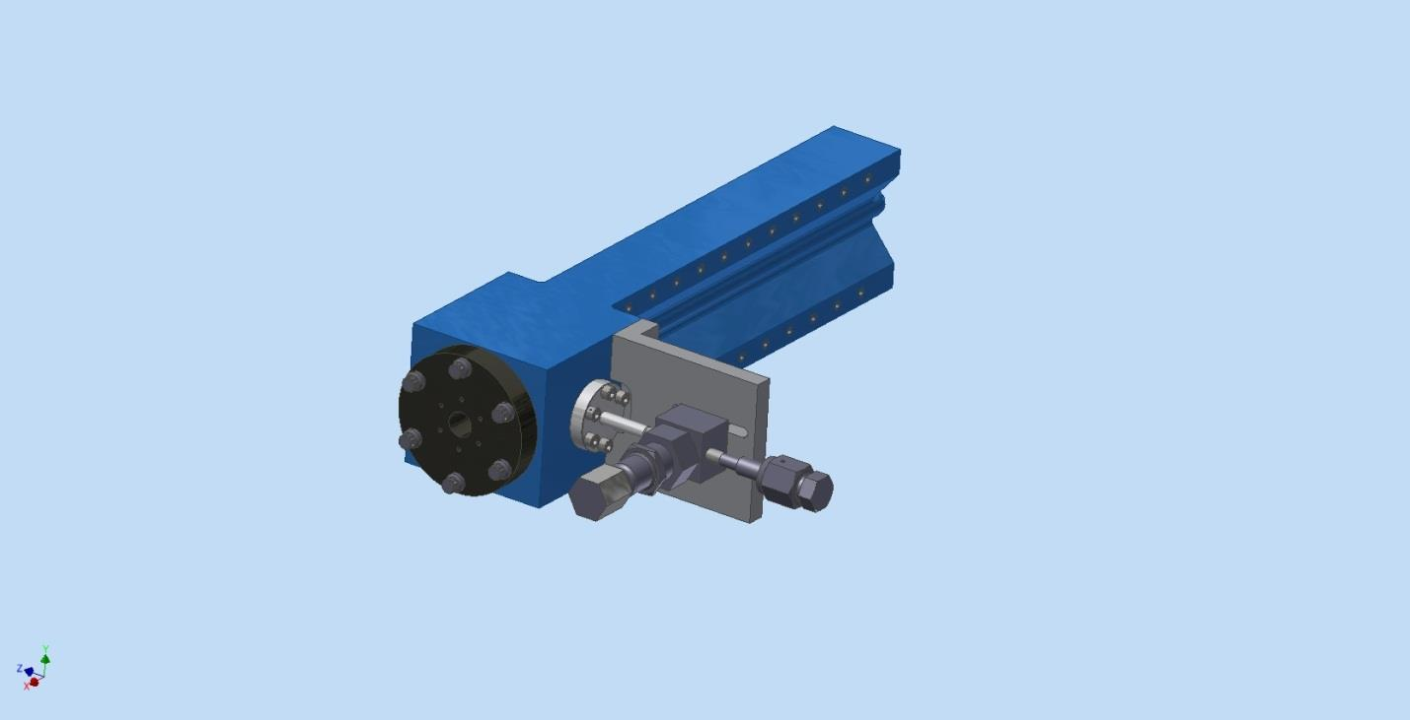
\includegraphics[width=0.7\textwidth]{./setup/fig/targ_cell.png}
	\caption{3D rendering of the target cell. The black circular plate in the front is the upstream window of the cell.\cite{cell_design}}
	\label{fig:3d_cell}
\end{center}
\end{figure}

The lack of gas circulation allows for localized heating of the gas in the cell. This is caused by the energy being deposited into the gas by the incident beam. The heating causes a density change in the gas changing the effective target thickness. This characteristic must be addressed in the analysis of gas target data and is discussed in further detail in Section \ref{sec:boiling}.

\subsection{Target Ladder}
The MARATHON target ladder can be seen in Figure \ref{fig:target}. This target ladder contained five targets that utilized the gas cell design described in the previous subsection. These are:
\begin{itemize}
	\item Tritium
	\item Deuterium
	\item Hydrogen
	\item Helium-3
	\item Empty Cell
\end{itemize}

The cells that contain gas (i.e. all of the above except the empty target) are used for studying the physics goals of the MARATHON experiment. In particular, Helium-3 and Deuterium are the focus of this thesis. Table \ref{tbl:gas_targs} lists the gas thicknesses and endcap thicknesses of the above gas targets.

\begin{table}[h]
\begin{tabular}{|l|c|c|c|}
\hline
Target & Gas Thickness $\nicefrac{\textrm{g}}{\textrm{cm}^2}$ & Entrance Window Thickness (mm) & Exit Window Thickness (mm) \\
\hline
\hline
Tritium & $77\pm0.01$ & $0.253\pm0.004$ & $0.3430.047$\\ \hline
Deuterium & $142.2\pm0.8$ & $0.215\pm0.004$ & $0.294\pm0.056$\\ \hline
Hydrogen & $70.8\pm0.4$ & $0.311\pm0.001$ & $0.330\pm0.063$\\ \hline
Helium-3 & $53.4\pm0.6$ & $0.203\pm0.007$ & $0.328\pm0.041$\\ \hline
Empty cell & $N/A$ & $0.254\pm0.0051$ & $0.279\pm0.0051$\\ \hline
\end{tabular}
\caption{Gas target thicknesses and cell wall thicknesses.\cite{targ_meas}}
\label{tbl:gas_targs}
\end{table}

In addition to the gas cells, the target ladder also contained several solid targets that are used for other studies. Those relevant to this thesis are:
\begin{itemize}
	\item 25cm Dummy
%	\item Optics Target - 11 Carbon Foils
	\item Carbon Hole - A carbon foil with a 2mm diameter hole in the center
	\item Raster Target - A ``straw'' for ensuring the beam is not coming in at an angle
%	\item Thick Aluminum - For calibrating the ion chambers
%	\item Single Carbon Foil
%	\item Titanium
%	\item Beryllium Oxide
\end{itemize}

\begin{figure}[h]
\begin{center}
	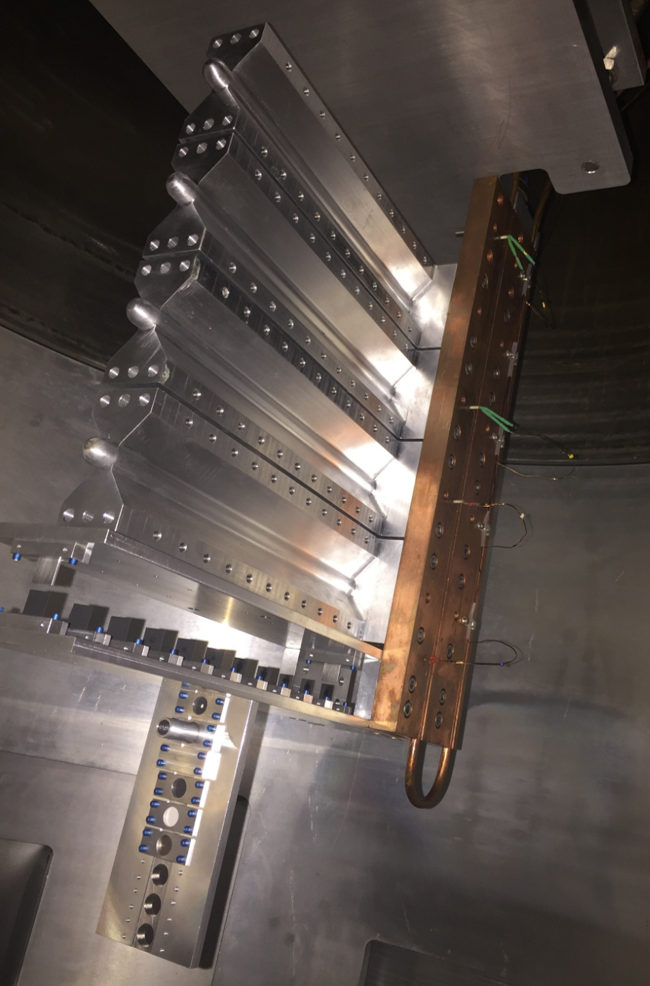
\includegraphics[width=0.4\textwidth]{./setup/fig/target.png}
	\label{fig:target}
	\caption{The MARATHON target ladder.}
\end{center}
\end{figure}

%Put in target data table: endcap thicknesses, density, fill pressure, target thickness

The Empty target is a gas cell that has a vacuum inside. The 25cm Dummy is comprised of two Aluminum 7075 foils, this is the same material as the gas cells. The foils are spaced 25cm apart, the same length as the gas cells.  Each foil is $0.3495\pm0.0006$ $g/cm^2$ thick, significantly thicker than the cell walls. These two targets are used to better understand the contribution of the gas cells to the electrons counted by the experiment. This study is discussed further in Section \ref{sec:ecc}.

The Carbon Hole target is a foil made of carbon that is $0.883\pm0.0002$ $g/cm^2$ thick with a $2mm$ diameter hole in the center. This target is used for centering the beam as well as for determining the settings needed for a $2mm$ by $2mm$ raster setting. This is also used to assist calibrating the raster as documented in Appendix \ref{app:raster_cal}.

After the beam is centered and the raster settings are determined, the Raster Target is used. This target is a ``straw'' that the beam should pass straight through. The goal of using this is to ensure that the beam is not approaching the target at an angle. If any counts are seen above background, then the beam is hitting the straw and can be assumed to be coming in at an angle that needs to be rectified. If the beam is angled, electrons would leave the physics targets before passing through all of the target material. This would significantly reduce counting rates and make it very difficult to determine the effective target thickness seen by the beam.